%%%%%%%%%%%%%%%%%%%%%%%%%%%%%%%%%%%%%%%%%%%%%%%%%%%%%%%%%%%%%%%%%%%%%%
% How to use writeLaTeX: 
%
% You edit the source code here on the left, and the preview on the
% right shows you the result within a few seconds.
%
% Bookmark this page and share the URL with your co-authors. They can
% edit at the same time!
%
% You can upload figures, bibliographies, custom classes and
% styles using the files menu.
%
%%%%%%%%%%%%%%%%%%%%%%%%%%%%%%%%%%%%%%%%%%%%%%%%%%%%%%%%%%%%%%%%%%%%%%

\documentclass[12pt]{article}

\usepackage{sbc-template}

\usepackage{graphicx,url}

%\usepackage[brazil]{babel}   
\usepackage[utf8]{inputenc} 

\usepackage{url}

%\usepackage{hyperref}
%\hypersetup{
%    colorlinks=false,
%    linkcolor=blue,
%    filecolor=magenta,      
%    urlcolor=cyan,
%}
     
\sloppy

\title{Instructions for Authors of SBC Conferences\\ Papers and Abstracts[Resumo e título são as ultimas partes de um artigo]}

\author{Frederico P. Antunes\inst{1}}


\address{Centro de Desenvolvimento Tecnológico – Universidade Federal de Pelotas (UFPel)\\
Pelotas – RS – Brazil
\email{fpantunes@inf.ufpel.edu.br}
}

\begin{document} 

\maketitle

\begin{abstract}
  This meta-paper describes the style to be used in articles and short papers
  for SBC conferences. For papers in English, you should add just an abstract
  while for the papers in Portuguese, we also ask for an abstract in
  Portuguese (``resumo''). In both cases, abstracts should not have more than
  10 lines and must be in the first page of the paper.
\end{abstract}
     
\begin{resumo} 
  [Resumo e título são as últimas partes de um artigo] Este meta-artigo descreve o estilo a ser usado na confecção de artigos e
  resumos de artigos para publicação nos anais das conferências organizadas
  pela SBC. É solicitada a escrita de resumo e abstract apenas para os artigos
  escritos em português. Artigos em inglês deverão apresentar apenas abstract.
  Nos dois casos, o autor deve tomar cuidado para que o resumo (e o abstract)
  não ultrapassem 10 linhas cada, sendo que ambos devem estar na primeira
  página do artigo.
\end{resumo}


\section{Introdução}

Cowichan, ou Problemas de Cowichan, é uma benchmark primeiramente desenvolvida em meados da década de 90 com o intuito de avaliar, e comparar, a usabilidade de sistema de programação paralelos e distribuídos, para a resolução de problemas pequenos que, porém, são análogos a problemas do mundo real e de tamanho mais considerável.

O desenvolvimento desse benchmark na década de 90 tem origem devido ao fato de que aproximadamente na mesma época houve um “boom” no tópico de processamento paralelo e distribuído, com um rápido crescimento no número de sistemas de programação paralela, e com o surgimento de processadores (CPUs) multicore e GPUs. Desde então essa área evoluiu e se expandiu ainda mais, com processadores multicore e GPUs se tornando praticamente ubíquos em computadores pessoais atuais, e tecnologias como o processamento na nuvem se tornando possível.

Com esse avanço na área, em 2010 o benchmark foi revisitado e reorganizado por Greg Wilson, para ser usado na avaliação da paralelização dos algoritmos com tecnologias e sistemas atuais. Assim são propostos 14 pequenos algoritmos, sendo esses chamados de toys, que trabalham com entradas de vetores e matrizes, e possuem variados graus de efetividade na implementação de paralelização neles.

Para esse trabalho, foi decidido implementar o toy de normalização da localização de pontos de uma matriz (Point Location Normalization), que utiliza uma pequena função matemática, sobre um vetor com as coordenadas de um ponto, para retornar essas coordenadas normalizadas entre 0 e 1. Sendo utilizado os sistemas Pthreads e OpenMP, implementados em C, para fazer a paralelização dessa função de normalização. Os códigos implementados pro trabalho podem ser encontrados em: \url{https://github.com/hpfred/}.

\section{Pthreads} \label{sec:firstpage}

Pthreads, ou POSIX Threads, é um padrão POSIX que possui uma interface de programação que permite criar e manipular threads, sendo thread um fluxo de processamento independente, dentro de um dado processo. Esse padrão foi desenvolvido numa época que linguagens orientadas a objeto estavam em sua infância, e não se via um maior nível de abstração como algo essencial, tendo então um foco maior em desempenho e em sua flexibilidade, dando ao programador maior controle sobre as características do paralelismo, tendo por consequência uma maior complexidade para programar, e relegando ao programador uma maior responsabilidade.

\section{OpenMP}

OpenMP, ou Open Multi-Processing, é uma interface de programação de aplicações concebida para explorar de forma eficiente o hardware paralelo. Para se alcançar essa melhor exploração do hardware, ele deve seguir um modelo mais eficiente pré estabelecido, fornecendo ao programador menos responsabilidade e uma maior abstração, mas tendo, por consequência, menos liberdade em como descrever a concorrência na aplicação. Uma das grandes vantagens dessa maior abstração da ferramenta é a extrema facilidade em estabelecer uma região paralela, e se fazer laços paralelamente, sendo laços perfeitos para paralelização, sendo eles trechos de código com imensa repetição normalmente usados para cálculos (que com a repetição podem se tornar rapidamente em cálculos computacionalmente exigentes) sem necessidade de acesso a uma memória compartilhada.

\section{Point Location Normalization}

O toy de normalização da localização de pontos, selecionado para ser implementado neste trabalho, tem a função de, como o nome indica, normalizar a localização de pontos de uma matriz. O que isso realmente significa é que para uma dada série de valores de entrada, cada par representa as coordenadas de um ponto e, após passar por um algoritmo de normalização, os valores da coordenada desse mesmo ponto serão um valor de no mínimo zero e no máximo um. 

Explicando de forma mais precisa, a função receberá como entrada um vetor possuindo a localização de diversos pontos, essa localização é representada por dois valores que dão a sua coordenada X e coordenada Y. A função, então, definirá os maiores e menores valores de ambas coordenadas, sendo esses valores definidos como Xmin, Xmax, Ymin e Ymax. Sabendo-se valores máximos e mínimos da matriz dos pontos, cada ponto terá suas coordenadas normalizadas seguindo o cálculo das seguintes equações:

\begin{equacao}

\centering Xi'    =    (Xi — Xmin)/(Xmax - Xmin)

\end{equacao}

\begin{equacao}

\centering Yi'    =    (Yi — Ymin)/(Ymax - Ymin)

\end{equacao}

Sendo Xi’ e Yi’ as coordenadas Xi e Yi, de um dado ponto, normalizadas.

Pode-se também dizer que qualquer coordenada maior que Xmax e Ymax, e menor que Xmin e Ymin, fazem parte da matriz onde estão descritos os pontos, mas não está descrita na matriz formada pelos pontos. Portanto a matriz normalizada é delimitada pelas maiores e menores coordenadas dos pontos, e por isso o resultado da normalização pode ser dito como uma porcentagem da matriz normalizada. Uma porcentagem dada entre a maior coordenada (1 ou 100\%) e menor coordenada (0 ou 0\%) de cada eixo.

O fato da coordenada normalizada ser equivalente a uma porcentagem é importante, pois ele permite compreender usos reais dessa função de normalização dos pontos. Um exemplo de uso da normalização é escalabilidade de resolução, por exemplo, se você tem uma imagem 4K e um monitor 1080p, a imagem não pode só mostrar 1/4 do seu conteúdo, então ela é redimensionada, perdendo alguns de seus pixels/pontos, mas mantendo a estrutura geral da imagem. De forma similar a imagem, outro exemplo é uma representação de uma coordenada geográfica em um mapa, se o GPS dá uma posição muito detalhada, o mapa deve conseguir normalizar essa coordenada para a sua escala, e apontar com a maior precisão possível a localização no mapa.

Dois exemplos simplificados desses uso podem ser observado nas Figuras ~\ref{fig:exampleFig1} e ~\ref{fig:exampleFig2}.

\begin{figure}[ht]
\centering
\includegraphics[width=1\textwidth]{50X25X10.png}
\caption{A typical figure}
\label{fig:exampleFig1}
\end{figure}

\begin{figure}[ht]
\centering
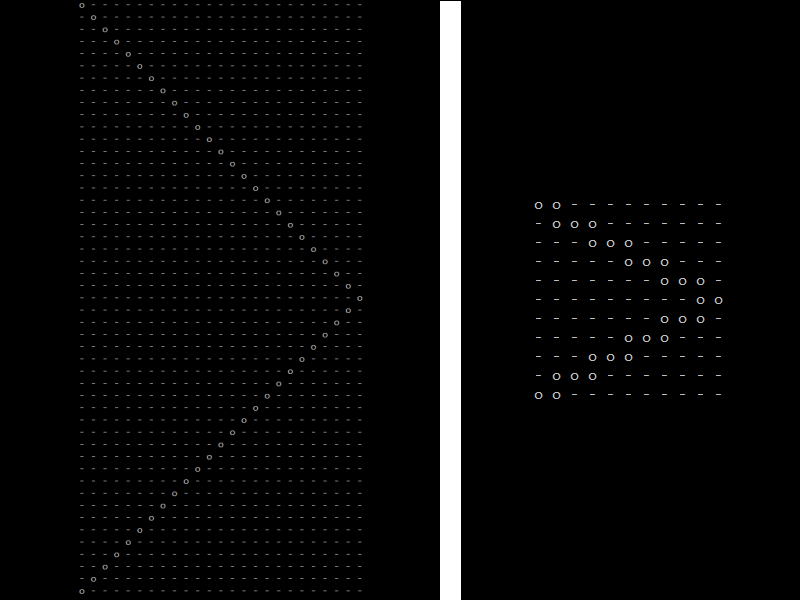
\includegraphics[width=.5\textwidth]{50.25x10.10.png}
\caption{A typical figure}
\label{fig:exampleFig2}
\end{figure}

\subsection{Subsections}

The subsection titles must be in boldface, 12pt, flush left.

\section{Figures and Captions}\label{sec:figs}


Figure and table captions should be centered if less than one line
(Figure~\ref{fig:exampleFig1}), otherwise justified and indented by 0.8cm on
both margins, as shown in Figure~\ref{fig:exampleFig2}. The caption font must
be Helvetica, 10 point, boldface, with 6 points of space before and after each
caption.

\begin{figure}[ht]
\centering
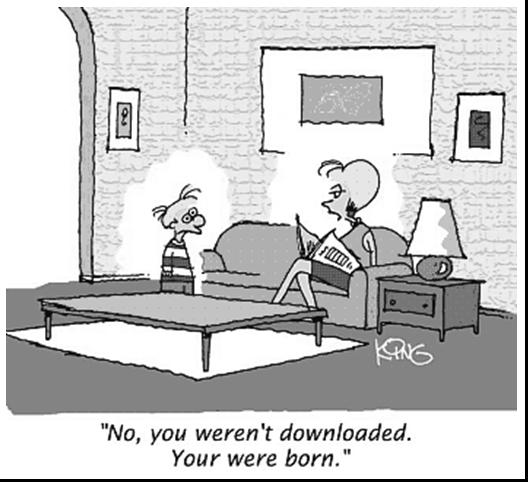
\includegraphics[width=.5\textwidth]{fig1.jpg}
\caption{A typical figure}
\label{fig:exampleFig3}
\end{figure}

\begin{figure}[ht]
\centering
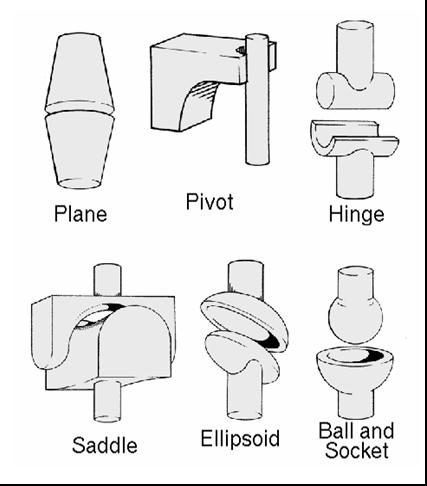
\includegraphics[width=.3\textwidth]{fig2.jpg}
\caption{This figure is an example of a figure caption taking more than one
  line and justified considering margins mentioned in Section~\ref{sec:figs}.}
\label{fig:exampleFig4}
\end{figure}

In tables, try to avoid the use of colored or shaded backgrounds, and avoid
thick, doubled, or unnecessary framing lines. When reporting empirical data,
do not use more decimal digits than warranted by their precision and
reproducibility. Table caption must be placed before the table (see Table 1)
and the font used must also be Helvetica, 10 point, boldface, with 6 points of
space before and after each caption.

\begin{table}[ht]
\centering
\caption{Variables to be considered on the evaluation of interaction
  techniques}
\label{tab:exTable1}
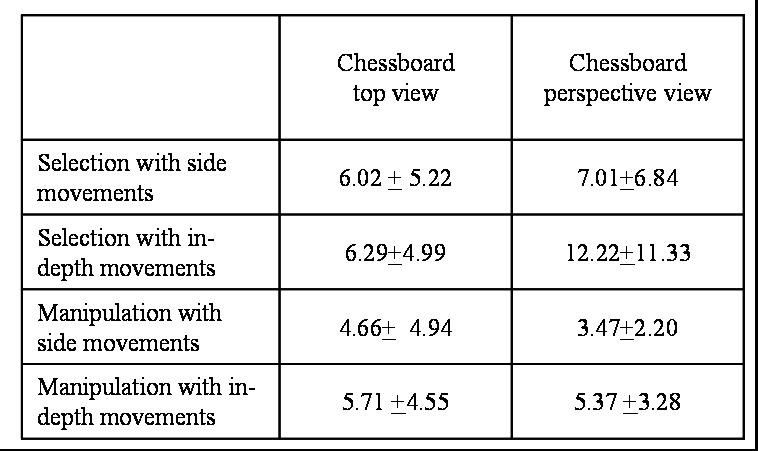
\includegraphics[width=.7\textwidth]{table.jpg}
\end{table}

\section{Images}

All images and illustrations should be in black-and-white, or gray tones,
excepting for the papers that will be electronically available (on CD-ROMs,
internet, etc.). The image resolution on paper should be about 600 dpi for
black-and-white images, and 150-300 dpi for grayscale images.  Do not include
images with excessive resolution, as they may take hours to print, without any
visible difference in the result. 

\section{References}

Bibliographic references must be unambiguous and uniform.  We recommend giving
the author names references in brackets, e.g. \cite{knuth:84},
\cite{boulic:91}, and \cite{smith:99}.

The references must be listed using 12 point font size, with 6 points of space
before each reference. The first line of each reference should not be
indented, while the subsequent should be indented by 0.5 cm.\cite{Wilson:94} \cite{Wilson:95}
\cite{Wilson:10} \cite{Kolmogorov} \cite{Howell:20}

\bibliographystyle{sbc}
\bibliography{sbc-template}

\end{document}
